\documentclass{tufte-handout}

%\geometry{showframe}% for debugging purposes -- displays the margins

\usepackage{amsmath}

% Set up the images/graphics package
\usepackage{graphicx}
\setkeys{Gin}{width=\linewidth,totalheight=\textheight,keepaspectratio}
\graphicspath{{graphics/}}

\title{Basics of Neuroendocrinology}
\author{Dave Bridges, Ph.D.}
%\date{24 January 2009}  % if the \date{} command is left out, the current date will be used

% The following package makes prettier tables.  We're all about the bling!
\usepackage{booktabs}

% The units package provides nice, non-stacked fractions and better spacing
% for units.
\usepackage{units}

% The fancyvrb package lets us customize the formatting of verbatim
% environments.  We use a slightly smaller font.
\usepackage{fancyvrb}
\fvset{fontsize=\normalsize}

% Small sections of multiple columns
\usepackage{multicol}

% Provides paragraphs of dummy text
\usepackage{lipsum}

% These commands are used to pretty-print LaTeX commands
\newcommand{\doccmd}[1]{\texttt{\textbackslash#1}}% command name -- adds backslash automatically
\newcommand{\docopt}[1]{\ensuremath{\langle}\textrm{\textit{#1}}\ensuremath{\rangle}}% optional command argument
\newcommand{\docarg}[1]{\textrm{\textit{#1}}}% (required) command argument
\newenvironment{docspec}{\begin{quote}\noindent}{\end{quote}}% command specification environment
\newcommand{\docenv}[1]{\textsf{#1}}% environment name
\newcommand{\docpkg}[1]{\texttt{#1}}% package name
\newcommand{\doccls}[1]{\texttt{#1}}% document class name
\newcommand{\docclsopt}[1]{\texttt{#1}}% document class option name

\begin{document}

\maketitle% this prints the handout title, author, and date

\begin{abstract}
\noindent The hypothalamus is the primary site of peripheral:central signal integration.  The two main parts of the brain that are involved in endocrine responses are the hypothalamus and the pituitary (Figure \ref{fig:pituitary-hypothalamus}).  This lecture will discuss the physical layout of these tissues and discuss how they communicate with each other, with the central nervous system and with peripheral signals.  This lecture will cover pages 333-335 and 508 in the textbook\cite{Widmaier2013}.

\begin{figure}[h]
  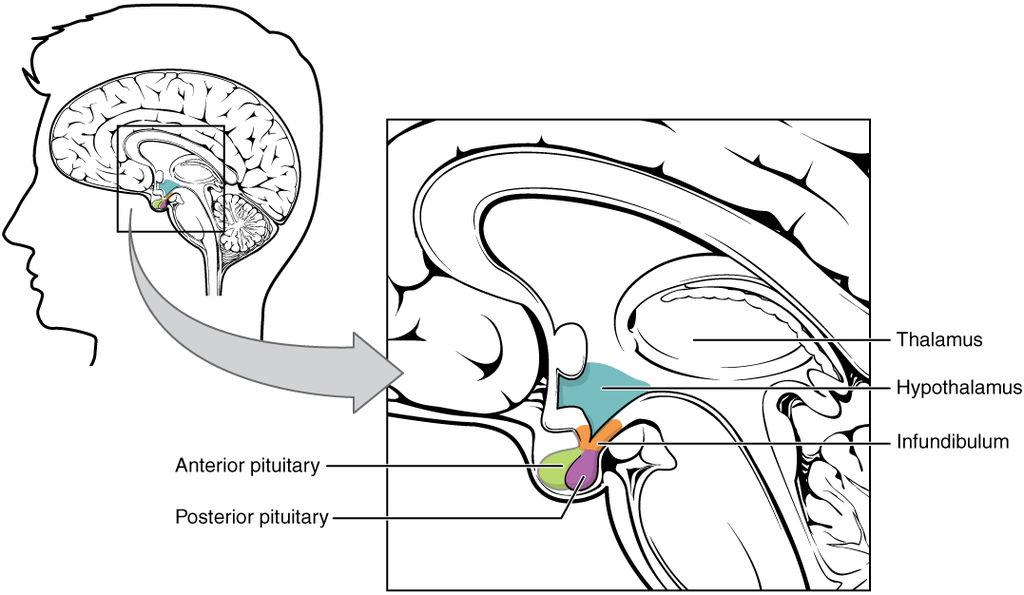
\includegraphics{figures/pituitary-hypothalamus}
  \caption{Location of the pituitary and hypothalamus in the human brain.}
    \label{fig:pituitary-hypothalamus}
\end{figure}
\end{abstract}

\tableofcontents

\pagebreak

\section{Learning Objectives}
For this lecture, the learning objectives are:
\begin{itemize}
\item Recall anatomical, biochemical, and functional evidence showing intimate relationships between hypothalamus and neurohypophysis.
\item Describe how hormones are sensed by the neurons of the hypothalamus, and the role that the blood brain barrier and transport mechanisms play.
\item Recall how the central nervous system can integrate with the hypothalamus and modify both hormonal secretions and executive function.
\item Describe the differences in how hypothalamic signals are passed to the posterior and anterior pituitary glands.
\item Name two major posterior pituitary hormones in man, name their chemical category, and succinctly describe their secretory mechanism.
\item Describe the physiological functions of vasopressin (VP, ADH) and oxytocin (OT).
\item Describe cellular actions of vasopressin in terms of site of actions, receptors, and cellular signals.
\item Discuss briefly aquaporin water channels and relation to vasopressin. 
\item Predict what the changes are expected in urine volume and osmolality and in ECF volume when vasopressin synthesis or secretion is severely impaired. Predict what will happen to water intake. Explain why there can be transient diabetes insipidus following a whiplash injury, and the rationale for therapy during this time. 
\item Describe the control of vasopressin release.
\item Describe the function of oxytocin with respect to delivery and lactation.


\end{itemize}

\pagebreak

\section{Anatomy of the Hypothalamus and Pituitary}

\subsection{The Hypothalamus}

The hypothalamus is located above the midbrain but below the thalamus.  It can respond to blood-borne signals because the blood-brain barrier is partially permeable in some regions.  Small hormones such as adrenaline, or lipid soluble hormones such as cortisol are able to permeate the barrier without assistance, but it has been proposed that some hormones are actively transported across the blood brain barrier to reach the hypothalamus \cite{Huber2001}.  The mechanisms of this differential permeability are not well understood, but for example resistance to the appetite suppressive effects of leptin in obesity are thought to, at least in part, be due to reduced leptin permeability \cite{Burguera2000}. 

\newthought{For such a small organ, the hypothalamus is very anatomically complex.}  The hypothalamus can be anatomically separated into several sub-regions called nuclei\sidenote{no these names will not be on the test}.  Each of these regions regulates a specific hypothalamic function, many of which will be covered in detail in future lectures.  As an example, the suprachiasmatic nucleus (SCN) regulates circadian rhythms which are the psychological, metabolic and behavioral changes that occur at approximately 24h cycles.  These internal hypothalamic nuclei can communicate with each other via direct neural projections.

\newthought{The hypothalamus connects to several other areas of the brain.}  In addition to its ability to communicate with the pituitary (see below), the hypothalamus also has bi-directional connections to other brain regions including the hippocampus, amygdala, prefrontal cortex.  In this way, direct neural connections between brain regions can form circuits in which internal signals, external signals and executive function can be combined.

\subsection{The Pituitary}

The Pituitary\sidenote{Named by Aelius Galenus in ~200 BC as the "gland that drops slime", due to a (incorrect) role in regulating nasal mucous} is a small pea-sized gland that is divided into three lobes, a posterior\sidenote{sometimes called the \emph{neurohypophysis}} , intermediate and anterior pituitary\sidenote{sometimes called the \emph{adenohyphosis}}.  The pituitary is located at the base of the brain, as shown in Figure \ref{fig:pituitary}.  The anterior pituitary produces and releases several hormones including growth hormone (GH), thyroid-stimulating hormone, adrenocorticotropic hormone (ACTH), prolactin, lutenizing hormone and folicle stimulating hormone (FSH).  These are released in response to signals from they hypothalamus, which pass through a specialized capillary system called the hypothalamic-hypophysial portal system.  The anterior pituitary is an extension of the hypothalamus and is responsible for the release of vasopressin and oxytocin, two peptide hormones. 

\begin{marginfigure}
  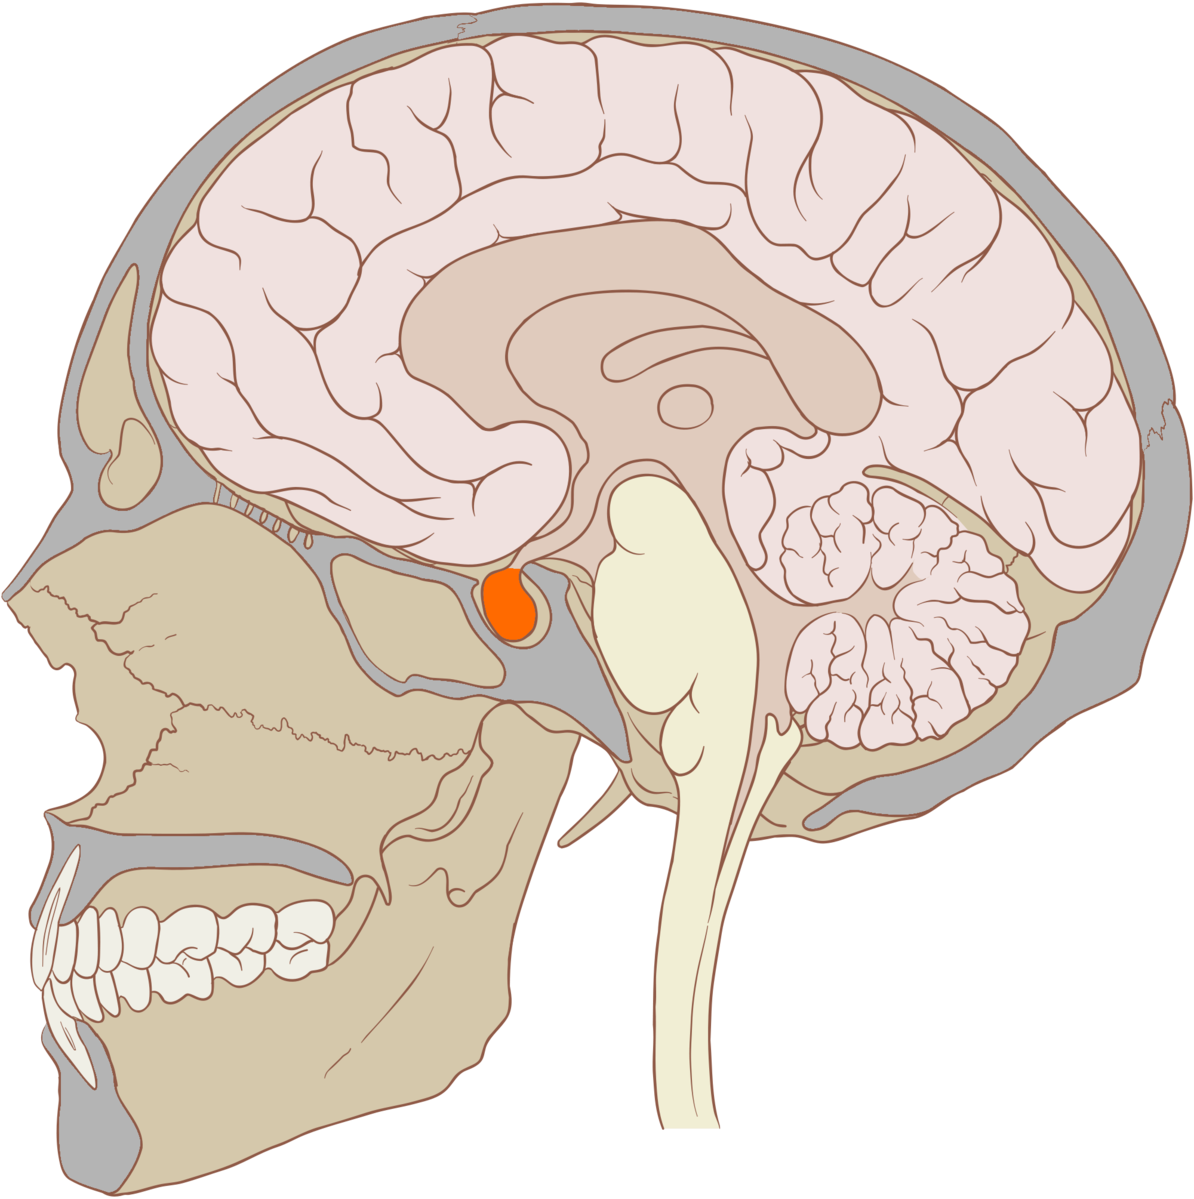
\includegraphics{figures/pituitary}
  \caption{The location of the pituitary.}
    \label{fig:pituitary}
\end{marginfigure}

\subsection{The Hypophyseal Portal System Connects the Hypothalamus to the Anterior Pituitary}

To communicate with the \emph{anterior pituitary}, hypothalamic neurons directly release hormones into a specialized blood vessel system called the hypophyseal portal system.  Hormones travel a small distance from the hypothalamus to the anterior pituitary\sidenote{These hormones are therefore at extremely low levels in the peripheral circulatory system and difficult to detect.}.  Here they bind to specific G-protein coupled receptors on specialized secretory cells of the anterior pituitary.  Specificity in these endocrine systems is achieved by having specialized cells, with specialized receptors which only respond to specific hypothalamic hormones and only secrete one substance into the peripheral circulation.  There are several examples of this system, described in Table \ref{tab:anterior-pituitary-hormones}.

\begin{table}
  \centering
  \begin{tabular}{ccc}
    \toprule
    Acronym & Hypothalamic Hormone & Pituitary Hormone \\
    \midrule
    CRH & Corticotropin Releasing Hormone & ACTH \\
    GnRH & Gonadotropin Releasing Hormone & FSH/LH\\
    TRH & Thyrotropin Releasing Hormone & TSH/Prolactin \\
    GHRH & Growth Hormone Releasing Hormone & GH \\
    SS & Somatostatin & Prevents GH \\
    \bottomrule
  \end{tabular}
  \caption{Hormones which use the hypophyseal portal system.}
  \label{tab:anterior-pituitary-hormones}
  %\zsavepos{pos:normaltab}
\end{table}


\subsection{The Infundibulum Connects the Hypothalamus to the Posterior Pituitary}

The posterior pituitary is an outgrowth of the hypothalamus and therefore has direct neural projections from the hypothalamus.  This anatomical structure is called the infundibulum and the neurons in this region initiate in the hypothalamus, but rather than releasing a neurotransmitter into a synapse, they directly release their hormones from their axons into the circulation.

\section{The Hormones of the Posterior Pituitary}

\subsection{Vasopressin}

Vasopressin\sidenote{occasionally called ADP (antidiuretic peptide), ADH (antidiuretic hormone), or argipressin} is a key component of the regulation of osmolality.  Elevated osmolality (too much salt in the blood) is sensed by osmoreceptors in the  paraventricular nuclei  and supraoptic nucleus of the hypothalamus.  Osmotic status is also sensed by other regions of the brain with permeable blood brain barriers such as the subfornicular organ, which then projects to the vasopressin releasing neurons in the hypothalamus.  Alternatively, a \emph{decrease} in blood volume can be detected by mechanoreceptors in the carotid sinus, which also project to the vasopressin-releasing neurons.  Once activate by one of these stimuli, these neurons release vasopressin into the blood stream.

\newthought{Vasopressin is sensed peripherally by 4 receptors.} The most important of these is AVPR2, which is a G$_s$-linked GPCR in the collecting ducts of the kidney.  This cascade activates PKA-mediated exocytosis of AQP2\sidenote{an aquaporin, or water transporter} containing vesicles, increasing the amount of AQP2 at the plasma membrane.  This allows for more water to be transported back from the collecting ducts into the blood.  This process is summarized in Figure \ref{fig:vasopressin}, modified from \cite{Verkman2014}.  An additional role of vasopressin is to cause modest vasoconstriction in the vasculature.  This occurs to reduce blood flow in the case that reduced blood volume is due to trauma.  A third location for vasopressin receptors is the anterior pituitary, where the corticotrope cells have AVPR1B or AVPR3 receptors, which initiate  ATCH/cortisol-dependent stress responses.

\begin{marginfigure}
  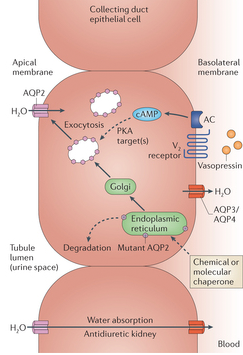
\includegraphics{figures/vasopressin}
  \caption{The role of vasopressin in kidney collecting ducts.}
    \label{fig:vasopressin}
\end{marginfigure}

\newthought{There are several disorders associated with abberant vasopressin signaling.}  Lack of vasopressin results in hypernatremia\sidenote{Elevated salt concentration in blood.} and diabetes insipidus\sidenote{thirst and release of excessive amounts of urine, not to be confused with diabetes mellitus which is a disorder of blood glucose levels.}.  This can be due to either lack of vasopressin production, or lack of response to vasopressin in the kidneys.  On the other hand, too much vasopressin signaling\sidenote{sometimes by a vasopressin-secreting tumor, or in response to nephrotic syndrome} can result in hyponatria.  This is often be treated by vasopressin antagonists.

\subsection{Oxytocin}

Like vasopressin, oxytocin is a peptide hormone released from the posterior pituitary.  The mechanisms which signal its release are not very well understood, but they involve synaptic activation of these neurons in the PVN of the hypothalamus.  In response to these signals, oxytocin is secreted at the posterior pituitary into the blood stream.

\newthought{The best characterized role of oxytocin is during delivery.}  The uterine wall responds to elevations in oxytocin to induce contractions.  Sensory neurons detect these contractions and project directly back to the brain where they synapse with the oxytocin releasing neurons.  This causes more oxytocin release and therefore forms a \emph{positive feedback loop} known as the Ferguson reflex\cite{Ferguson1941}.

Another role of oxytocin is in the release of milk at mammary glands.  Oxytocin release stimulates contraction of the smooth muscle that lines the mammary alveoli releasing the milk into the mammary ducts.  In this manner it works alongside prolactin\sidenote{Prolactin stimulates the production of milk} to ensure proper production and release of milk.  Even less well understood is the effects of oxytocin on mood and behavior.  Oxytocin has been linked to enhanced feelings of trust, social interactivity and bonding through neuroendocrine mechanisms that are just being explored now.

\listoffigures
\listoftables

\bibliography{library}
\bibliographystyle{plainnat}



\end{document}
